\documentclass[tikz,14pt,fleqn]{article}


\usepackage[utf8]{inputenc}
\usepackage[margin=1in]{geometry}
\usepackage[titletoc,title]{appendix}
\usepackage{latexsym}
\usepackage{amssymb}
\usepackage{gensymb}
\usepackage{amsmath}
\usepackage{amsfonts}
\usepackage[dvipsnames]{xcolor}
\usepackage{multicol}
\usepackage{graphicx}
\usepackage{fancyhdr}
\usepackage[linguistics]{forest}
\usepackage{colortbl}
\usepackage{pdfpages}
\usepackage{wrapfig}
\usepackage{cleveref}
\usepackage{cancel}
\usepackage{multirow}

% to fixme
\usepackage{xcolor} 
\definecolor{FIXMECOLOR}{rgb}{1,0,0}
\newcommand{\FIXME}[1]{{\color{FIXMECOLOR}{\textbf{FIXME: #1}}}} 

% to simplify math 
\newcommand{\pvec}[3]{
   \ensuremath{
   \begin{pmatrix}
       #1 \\
       #2 \\
       #3
   \end{pmatrix}
}}

\newcommand{\bvec}[3]{
   \ensuremath{
   \begin{bmatrix}
       #1 \\
       #2 \\
       #3
   \end{bmatrix}
}}

\newcommand{\bmat}[1]{
   \ensuremath{
   \begin{bmatrix}
       #1
   \end{bmatrix}
}}

\newcommand{\dotprod}[2]{\ensuremath{\left< #1, #2 \right>}}

%% For plotting
\usepackage{pgfplots}
\pgfplotsset{width=10cm,compat=1.9}
\usepgfplotslibrary{external}
\tikzexternalize
%%
\usepackage{dirtree}
\usepackage{subcaption}
\usepackage{xifthen}% provides \isempty test
\usepackage{glossaries}

\captionsetup[subfigure]{labelformat=empty}
\definecolor{color1}{HTML}{0B0C10}
\definecolor{color2}{HTML}{1F2833}
\definecolor{color3}{HTML}{C5C6C7}
\definecolor{color4}{HTML}{66FCF1}
\definecolor{color5}{HTML}{45A29E}

\pagestyle{fancy}
\fancyhf{}
%%%%%%%%%%%%%%%%%%%%%%%%%%%%
%% VARIABLES
\newcommand\namesurname{Albert Cerfeda\\Alessandro Gobbetti}
\newcommand\assignment{Assignment 7}

\newcommand\subject{Computer Graphics}
\newcommand\documentdate{10.11.2022}

% Title content
%%%%%%%%%%%%%%%%%%%%%%%%%%%%
\rhead{\assignment}
\lhead{\namesurname}
%%%%%%%%%%%%%%%%%%%%%%%%%%%%
\rfoot{Page \thepage}
\setlength{\parindent}{0pt}

\newcommand\xdownarrow[1][2ex]{%
   \mathrel{\rotatebox{90}{$\xleftarrow{\rule{#1}{0pt}}$}}
}

\begin{document}

\begin{titlepage}
   \begin{center}
       \vspace*{1cm}

       \textbf{\Large{Homework Assignment}}

       \vspace{0.5cm}
        \textbf{\subject}\\[5mm]
       \assignment
        
            
       \vspace{1.8cm}

        \namesurname
       \tableofcontents

       \vspace*{\fill}
     
        
\includegraphics[width=0.4\textwidth]{fig/logo.png}
       
        \documentdate \\
        Università della Svizzera italiana\\
        Faculty of Informatics\\
        Switzerland\\

   \end{center}
\end{titlepage}



\section{Exercise 1}
Considering the camera opening angle be $\pi/2$ radians and the image be 10 × 10 pixels large. Consider the camera in the origin and the image plane at z-coordinate 1.
Thus, the top-right image corner will be at coordinates $(1,1,1)$ and the bottom left one will be at $(-1,-1,1)$. 


Consider the line $l$ from $p_1 = (-1, -1, 2)$ to $p_2 = (7, 1, 10)$.

Lets consider now the rays from $p_1$ and $p_2$ to the origin (the camera position) and compute intersections $q_1$ and $q_2$ with the image plane.



\[
q_1 = (-0.5, -0.5), \quad q_2 = (\frac{7}{10}, \frac{1}{10})=(0.7,0.1)
\]

If we consider that we index pixels starting from top-left corner, i.e.,
the top-left pixel has indices (1, 1) and the bottom-right one (10, 10), We can convert $q_1$ and $q_2$ to image coordinates:
\[
q_1 = (3,8), \quad
q_2 = (9,5)
\]

The midpoint algorithm uses solves the problem of representing a line on screen pixels by considering midpoints between pixels and decide which pixel turn on based on the position of the midpoints in respect to the line.

\begin{figure}[h!]
    \centering
    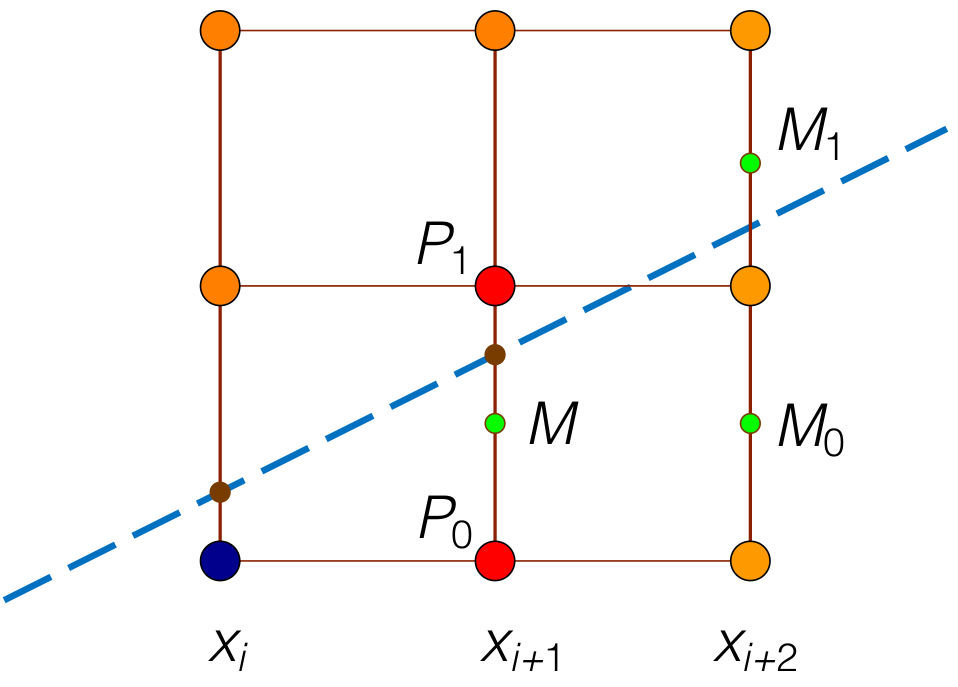
\includegraphics[width=0.4\textwidth]{fig/midpoint_alg.png}
    \caption{Midpoint algorithm.}
    \label{fig:midpoint}
\end{figure}
In each $x$-step, there are two options for the $y$-coordinate: it stays as it is (same row of pixel) or it increases by one (one row higher).

We can compute midpoint decider incrementally (since in our coordinate system y axis is inverted, we  have to invert ys):
\[
F(M_0) = F(M) +d_y
\]
\[
F(M_1) = F(M) +d_y + d_x
\]
With initial value $F(M) = +d_y + d_x/2 = +(-(5-8)) + (9-3)/2 = -3+6/2 = 0$.

So, until we reach $q_2$:

\begin{tabular}{ll}
    $F(M_0) = 0 -3 = -3 < 0$ &  \multirow{2}{*}{$(x, y)$ lies below the line and thus we choose (4,8)}\\
    $F(M_1) = 0 -3 + 6= 3 > 0$ & 
\end{tabular}

% \[
% F(M_0) = -3 -3 = -6 < 0,  \qquad
% F(M_1) = -3 -3 + 6= 0 > 0, \qquad \text{$(x, y)$ lies above the line and thus we choose (4,8)}
% \]
After (4,8):

\begin{tabular}{ll}
    $F(M_0) = -3 -3 = -6 < 0$ &  \multirow{2}{*}{(x, y) lies on the line, we choose (5,7)}\\
    $F(M_1) = -3 -3 + 6= 0 = 0$ & 
\end{tabular}

% \[
% F(M_0) = 3 -3 = 0 = 0,  \qquad
% F(M_1) = 3 -3 + 6= 6 > 0, \qquad \text{(x, y) lies on the line, we choose (5,7)}
% \]

After (5,7):

\begin{tabular}{ll}
    $F(M_0) = 0 -3 = -3 < 0$ &  \multirow{2}{*}{we choose (6,7)}\\
    $F(M_1) = 0 -3 + 6= 3 > 0$ & 
\end{tabular}
% \[
% F(M_0) = 0 -3 = -3 < 0,  \qquad
% F(M_1) = 0 -3 + 6= 3 > 0, \qquad \text{we choose (6,7)}
% \]

After (6,7):

\begin{tabular}{ll}
    $F(M_0) = -3 -3 = -6 < 0 $ &  \multirow{2}{*}{we choose (7,6)}\\
    $F(M_1) = -3 -3 + 6= 0 = 0$ & 
\end{tabular}
% \[
% F(M_0) = 3 -3 = 0 = 0,  \qquad
% F(M_1) = 3 -3 + 6= 6 > 0, \qquad \text{we choose (7,6)}
% \]

After (7,6):

\begin{tabular}{ll}d
    $F(M_0) = 0 -3 = -3 < 0$ &  \multirow{2}{*}{we choose (8,6)}\\
    $F(M_1) = 0 -3 + 6= 3 > 0$ & 
\end{tabular}
% \[
% F(M_0) = 0 -3 = -3 < 0,  \qquad
% F(M_1) = 0 -3 + 6= 3 > 0, \qquad \text{we choose (8,6)}
% \]

After (8,6):

\begin{tabular}{ll}
    $F(M_0) = -3 -3 = -6 < 0$ &  \multirow{2}{*}{we choose (9,5)= $q_2$}\\
    $F(M_1) = -3 -3 + 6= 0 = 0$  & 
\end{tabular}
% \[
% F(M_0) = 3 -3 = 0 = 0,  \qquad
% F(M_1) = 3 -3 + 6= 6 > 0, \qquad \text{we choose (9,5)= $q_2$}
% \]


To recap, the line on the image will be represented by the pixels:
(3,8), (4,8), (5,7), (6,7), (7,6), (8,6), (9,5).

\subsection*{a)}
The middle pixel (along the horizontal direction) of the line is $m = (6,7)$.
Since $m$ is exactly in the middle between $q_1$ and $q_2$, $m$ will be also in the middle between $p_1 = (-1,-1,-1)$ and $p_2 = (7,1,10)$.
Thus:

\[
p^z = \frac{1}{(1-\lambda)\frac{1}{p_1^z}+\lambda\frac{1}{p_2^z}}
 = \frac{1}{\frac{1}{2}\frac{1}{2}+\frac{1}{2}\frac{1}{10}} = \frac{1}{\frac{1}{4}+\frac{1}{20}} =  \frac{1}{\frac{6}{20}} = \frac{1}{\frac{3}{10}} = \frac{10}{3} \approx 3.33
\]



\subsection*{b)}
Assuming that the $p_1$ should be rendered in red, $rgb = (1, 0, 0)$, and $p_2$ in green, $rgb = (0, 1, 0)$,
the middle point will be colored $rgb = (1\cdot0.5 + 0\cdot0.5, 0\cdot0.5 + 1\cdot0.5, 0) = (0.5, 0.5, 0)$.

\[
A = \frac{(1-\lambda)\frac{A_1}{p_1^z}+\lambda\frac{A_2}{p_2^z}}{\frac{1}{p^z}}
= \frac{(1-\frac{1}{2})\frac{A_1}{2}+\frac{1}{2}\frac{A_2}{10}}{\frac{1}{\frac{10}{3}}}
= \frac{\frac{1}{2}\frac{(1, 0, 0)}{2}+\frac{1}{2}\frac{(0,1,0)}{10}}{\frac{3}{10}}
= \frac{\frac{1}{4}(1, 0, 0)+\frac{1}{20}(0, 1, 0)}{\frac{3}{10}}
= \frac{(\frac{1}{4},\frac{1}{20},0)}{\frac{10}{3}}
= (\frac{5}{6},\frac{1}{6},0)
\]

\section{Exercise 2}
Knowing the three vertices of the triangle we can divide the mesh into two separate subtriangles such that we get an horizontal cut in the primary mesh that goes through $p_1$.

Now we can consider the two triangles separately. We can construct a bounding-box for each subtriangle and iterate the pixels from left to right, bottom to top.\\

Barycentric coordinates have properties that are helpful to us, ie:
\begin{itemize}
\item The sum of all barycentric coordinates is always $1$\\
\item The ratio of all the areas of the subtriangles created by the point lying inside/outside of the mesh is \textbf{constant}.
\end{itemize}

Consider now the horizontal edge of the triangle. The left vertex has barycentric coordinate (1,0,0) and the right one (0,0,1). We can linearly get the barycentric coordinates of the pixels in between knowing the width of the bounding box. The barycentric coordinate\\ related to the top vertex will stay 0.\\
When handling each pixel, we can calculate the ratio between the position of the pixel relatively to the bounding-box width/height, and use it to adjust the barycentric coordinates accordingly. 
% We can now move to the pixel row above we can compute the new barycentric coordinate associated with the new height. The 
\end{document}

